\chapter{Jupyter Notebooks, APIs and Servers}

%==============================================================================
%
%==============================================================================
\section{Introduction to Jupyter Notebooks}

%==============================================================================
%
%==============================================================================
\subsection{What is Jupyter Notebook?}


Jupyter Notebook is an open-source web-based tool that allows you to create and share documents containing live code, equations, visualizations, and explanatory text. It supports various programming languages, including Python, making it an essential tool for data analysis, machine learning, and scientific computing. Its interactive nature allows for rapid prototyping, testing, and visualization of code, making it particularly useful for beginners and experts alike.

%==============================================================================
%
%==============================================================================
\subsection{Installing and Running Jupyter}

To install Jupyter Notebook, use Python’s package manager, \texttt{pip}:

\begin{codeonly}{Install Jupyter Notebook}
pip install jupyter
pip install jupysterlab
\end{codeonly}

Once installed, you can start Jupyter Notebook by running the following command in your terminal:

\begin{codeonly}{Run Jupyter Notebook}
jupyter notebook
\end{codeonly}

or \texttt{jupyter notebook mynotebook.ipynb}. This will open a web browser with the Jupyter interface, allowing you to create and manage notebooks. On many clouds there is jupyter pre-installed with many packages which you might want to use. 

As an example, Amazon Web Services (AWS) for example offers a ready-to-go machine learning framework where you get all packages for using pytorch from the beginning. However, running any of these will cost you per hour - do not forget to shut it down once you are done, otherwise you might be surprised how small amounts of payments can accumulate over days and weeks (happened to me once). 

%==============================================================================
%
%==============================================================================
\subsection{Basic Operations in Jupyter}

In Jupyter, each notebook consists of cells that can hold code, text, or markdown. Common operations include:

\begin{itemize}
    \item \bbb{Running Code:} Press \texttt{Shift+Enter} to execute the code in the current cell and move to the next.
    \item \bbb{Adding Cells:} Use the \texttt{+} button or press \texttt{B} to add a cell below the current one.
    \item \bbb{Changing Cell Type:} Switch between \texttt{Code} and \texttt{Markdown} using the dropdown or press \texttt{Esc + M}.
    \item \bbb{Saving Notebooks:} Press \texttt{Ctrl+S} or use the \texttt{Save} button to save your work.
		\item \bbb{Export as Code:} You can export a Jupyter Notebook to a Python code file by selecting \texttt{File > Download as > Python (.py)} in the Jupyter interface, or by running the command \texttt{jupyter nbconvert --to script notebook.ipynb} in the terminal.
\end{itemize}

Jupyter also provides built-in visualization support with libraries like \texttt{matplotlib}, making it ideal for data-driven projects. Its flexibility and ease of use make it a crucial tool for Python developers.

%==============================================================================
%
%==============================================================================
\subsection{Installing Packages in Jupyter Notebooks with \texttt{!pip install}}

In Jupyter Notebooks, you can install Python packages directly from within a code cell using the exclamation mark (\texttt{!}) followed by the usual \texttt{pip install} command. This is particularly useful because it eliminates the need to switch to a terminal or command line interface. The packages go into the virtual environment you have been using to call jupyter. 

To install a package, simply run:

\begin{codeonly}{Installing a Package in Jupyter}
!pip install numpy
\end{codeonly}

This command installs the \texttt{numpy} package in your current Jupyter environment.

\textbf{Why use \texttt{!pip install} in Jupyter?}
\begin{itemize}
    \item It ensures that the package is installed directly into the environment where the notebook is running.
    \item Convenient for interactive development without leaving the notebook interface.
\end{itemize}

If you encounter issues where Jupyter uses a different Python environment than your terminal, you can explicitly install packages to the notebook's Python environment by using:

\begin{codeonly}{Ensuring Correct Environment}
import sys
!{sys.executable} -m pip install package_name
\end{codeonly}

where
\begin{lstlisting}
print({sys.executable})
\end{lstlisting}
shows the path of the current python binary used for execution, i.e.

\begin{lstlisting}
{'C:\\Users\\rolan\\all\\ropy312\\Scripts\\python.exe'}
\end{lstlisting}
on my windows computer. 

This guarantees that \texttt{pip} installs the package into the environment running the notebook, ensuring compatibility and avoiding common environment issues.

%==============================================================================
%
%==============================================================================
\subsection{Running Jupyter on a Remote Linux Machine with Port Forwarding}

When working on remote servers, such as a Linux machine over SSH, you can still use Jupyter Notebooks by starting it on the remote machine and forwarding the port to your local machine (Windows or Linux). This ensures you can access the notebook in your local browser while running the code on the powerful remote server.

\subsubsection{Starting Jupyter on the Remote Linux Machine}

First, log in to your remote Linux machine via SSH. Then, start Jupyter Notebook with:
\begin{codeonly}{Remote Command on Linux}
jupyter notebook --no-browser --port=8888
\end{codeonly}

This command starts Jupyter on port \texttt{8888} without opening a browser window on the remote machine.

\subsubsection{Port Forwarding from Local Machine}

To access this remote Jupyter server, you need to forward the port from the remote machine to your local machine.
On a local Linux machine (using Bash) or Windows (Powershell):
\begin{codeonly}{Port Forwarding on Linux}
ssh -N -L 9001:localhost:8888 user@remote-server-ip &
\end{codeonly}

This forwards the remote port \texttt{8888} to your local machine’s port \texttt{9001}.


\subsubsection{Accessing Jupyter Notebook in Your Local Browser}

Once the SSH connection is established, open a browser on your local machine and navigate to:
\begin{verbatim}
http://localhost:9001
\end{verbatim}

You will see the Jupyter Notebook interface running on the remote machine, accessible from your local browser. However, it will probably ask you for the token, which is displayed when you start the Jupyter notebook: 

\begin{lstlisting}
    To access the server, open this file in a browser:
        file:///home/roland/.local/share/jupyter/runtime/jpserver-6745-open.html
    Or copy and paste one of these URLs:
        http://localhost:8888/tree?token=2bfafead00bd642b4fc56a57864e3e9ca92bc41e49f4c1f6
        http://127.0.0.1:8888/tree?token=2bfafead00bd642b4fc56a57864e3e9ca92bc41e49f4c1f6
\end{lstlisting}

The port 8888, however, is on the remote machine, you have forwarded it locally to 9001 and need to replace this, then use your browser to access the Jupyter notebook. 

%==============================================================================
%
%==============================================================================
\subsection{Using Markdown Cells for Documentation}

Markdown cells in Jupyter Notebooks allow you to add formatted text, making your notebooks more readable and well-documented. To create a Markdown cell, simply change the cell type from \texttt{Code} to \texttt{Markdown}.

Markdown supports:
\begin{itemize}
    \item \bbb{Headings:} Use \texttt{\#} for headings (\texttt{\# Heading 1}, \texttt{\#\# Heading 2}).
    \item \bbb{Bold and Italics:} Use \texttt{**bold**} or \texttt{*italic*}.
    \item \bbb{Lists:} Create ordered lists with numbers and unordered lists with dashes.
    \item \bbb{Links and Images:} Add links with \texttt{[text](url)} and images with \texttt{![alt text](image\_url)}.
    \item \bbb{LaTeX Equations:} For mathematical expressions, enclose LaTeX code in \texttt{\$...\$} for inline equations or \texttt{\$\$...\$\$} for display equations.
\end{itemize}

Markdown transforms Jupyter notebooks into interactive documents combining code, text, and visuals seamlessly.

%==============================================================================
%
%==============================================================================
\subsection{Using Magic Commands in Jupyter Notebooks}

Jupyter provides special \bbb{magic commands} that simplify various tasks such as timing code execution, managing the environment, and more. Magic commands start with a single \texttt{\%} for line magics and \texttt{\%\%} for cell magics.

\textbf{Common Magic Commands:}
\begin{itemize}
    \item \texttt{\%time}: Times the execution of a single line of code.
    \begin{codeonly}{Timing a Code Line}
%time sum(range(1000000))
    \end{codeonly}
    \item \texttt{\%timeit}: Runs code multiple times and gives an average runtime.
    \item \texttt{\%lsmagic}: Lists all available magic commands.
    \item \texttt{\%\%writefile}: Writes the contents of a cell to an external file.
\begin{codeonly}{Writing to a File}
%%writefile magic_hello.py
print("Hello, world!")
\end{codeonly}
    \item \texttt{\%\%bash}: Runs Bash commands directly inside a Jupyter cell.
\end{itemize}

Magic commands enhance productivity by providing quick, built-in operations within Jupyter.

%==============================================================================
%
%==============================================================================
\subsection{Running Shell Commands in Jupyter Notebooks}

Jupyter allows you to execute shell commands directly within code cells using the exclamation mark (\texttt{!}). This is useful for interacting with the operating system without leaving the notebook.

\textbf{Examples of Shell Commands in Jupyter:}
\begin{itemize}
    \item List files in the current directory:
    \begin{codeonly}{List Files}
!ls
    \end{codeonly}
    \item Install packages using \texttt{pip}:
    \begin{codeonly}{Install a Package}
!pip install numpy
    \end{codeonly}
    \item Check the Python version:
    \begin{codeonly}{Check Python Version}
!python --version
    \end{codeonly}
\end{itemize}

Shell commands allow seamless interaction with the system, making Jupyter highly versatile for both coding and administrative tasks.

%==============================================================================
%
%==============================================================================
\subsection{Data Visualization in Jupyter with Matplotlib, Seaborn, and Plotly}

Jupyter Notebooks integrate well with popular Python visualization libraries, making it easy to create plots and graphs directly within your notebook.

\begin{codeonly}{Lorenz63 Calculation and Visualization}
import numpy as np
import matplotlib.pyplot as plt

# Parameters and initial condition
sigma, beta, rho = 10, 8/3, 28
dt, steps = 0.01, 10000
xyz = np.empty((steps, 3))
xyz[0] = (1, 1, 1)

# Integration using Euler method
for i in range(steps - 1):
    x, y, z = xyz[i]
    dx = sigma * (y - x)
    dy = x * (rho - z) - y
    dz = x * y - beta * z
    xyz[i + 1] = xyz[i] + dt * np.array([dx, dy, dz])

# Plot the result
fig = plt.figure(figsize=(6, 4))
ax = fig.add_subplot(projection='3d')
ax.plot(*xyz.T, lw=0.5)
ax.set_title("Lorenz Attractor")
ax.set_facecolor("white")       # plot area (axes background)
plt.savefig('images/lorenz63.png')
plt.show()
\end{codeonly}

\begin{center}
\begin{figure}[ht]
   \centerline{
\includegraphics[width=0.8\textwidth]{images/lorenz63.png}}
	 \caption{Matplotlib within Jupyter, Lorenz 63 Attractor.}
\end{figure}
\end{center}%

And another code based on the seaborne package, where you need to \texttt{pip install seaborn} first, then run: 

\begin{codeonly}{lorenz63-seaborn.py}
import numpy as np
import matplotlib.pyplot as plt
import seaborn as sns

# Parameters for the Lorenz system
s = 10.0   # Sigma
r = 28.0   # Rho
b = 8.0 / 3.0  # Beta

# Time step and number of iterations
dt, N = 0.01, 10000

# Array to hold x, y, z
xyz = np.zeros((N, 3))
xyz[0] = 1, 1, 1  # Initial condition

# Integrate using Euler's method
for i in range(1, N):
    x, y, z = xyz[i-1]
    dx = s * (y - x)
    dy = x * (r - z) - y
    dz = x * y - b * z
    xyz[i] = x + dt * dx, y + dt * dy, z + dt * dz

# KDE plot with seaborn
sns.set(style="white")
plt.figure(figsize=(6, 5))
kde = sns.kdeplot(
    x=xyz[:, 0], y=xyz[:, 2],  # x vs z
    fill=True, cmap="viridis", levels=100, thresh=0.02
)
plt.colorbar(kde.collections[0], label="Density")
plt.title("Lorenz Attractor Density (x vs z)")
plt.xlabel("x")
plt.ylabel("z")
plt.tight_layout()
plt.savefig("images/lorenz63-seaborn.png")
plt.show()
\end{codeonly}

\begin{center}
\begin{figure}[ht]
   
\includegraphics[width=0.35\textwidth]{images/lorenz63-seaborn.png}
   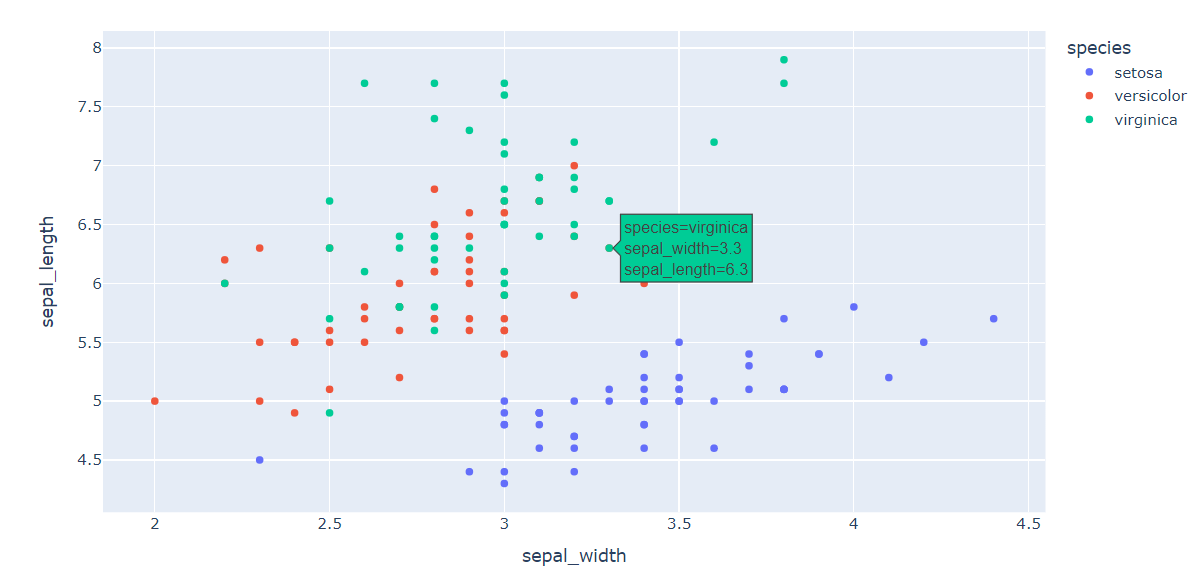
\includegraphics[width=0.6\textwidth]{images/plotly_interactive.png}
	\caption{Density visualization based on seaborne package and interactive plotly visualization.}
\end{figure}
\end{center}%

Interactive plots can easily be integrated into jupyter notebooks, here for example with the \emph{plotly} package. You need to install
\begin{lstlisting}
pip install numpy
pip install plotly
pip install pandas
\end{lstlisting}
We will discuss pandas further in a later session. 

\textbf{Using \texttt{plotly} for Interactive Plots:}
\begin{codeonly}{Plotly Example}
import plotly.express as px
df = px.data.iris()
fig = px.scatter(df, x='sepal_width', y='sepal_length', color='species')
fig.show()
\end{codeonly}

With these and further libraries, Jupyter becomes a powerful tool for both static and interactive data visualizations. You cannot develop applications in artificial intelligence without looking at data and results in a very careful way, bringing in a lot of domain specific know-how! 

\begin{recommendationbox}
Fluency in using Jupyter Notebooks is essential for effective Python development. 
\end{recommendationbox}


%==============================================================================
%
%==============================================================================
\section{Introduction to APIs: A Key Principle in Code Development}

Python is more than a programming language. It is an eco system which provides a lot of functionality which is needed for either AI/ML applications or other types of user services. In particular, APIs are extremly useful and, today, ubiquitous in scientific applications. 

An \bbb{API (Application Programming Interface)} is a defined set of rules and tools that allows different pieces of software to communicate with each other. APIs are essential in modern programming because they enable modular, reusable, and maintainable code. From simple functions within a local Python module to complex web-based services, APIs provide a structured way to access and share functionality.

\begin{center}
\begin{figure}[ht]
   \centerline{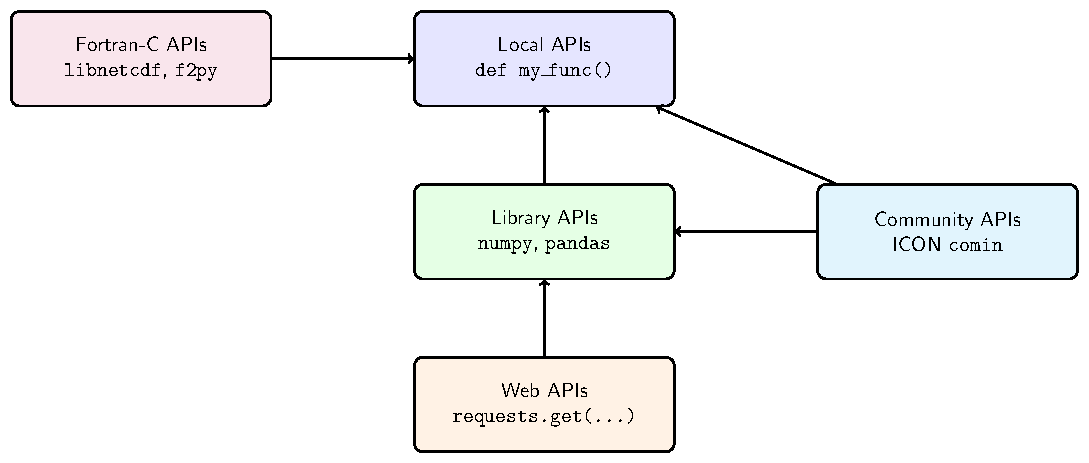
\includegraphics[width=0.8\textwidth]{chapters/api_diagram.pdf}}
	\caption{Importance of API design and functionality.}
\end{figure}
\end{center}%

APIs work by exposing specific methods or endpoints that other code can call. For example, a Python module can expose a function like \texttt{add(a, b)}, or a web service can expose an HTTP endpoint like \texttt{/weather?city=Berlin}. In both cases, the underlying logic is hidden, and only the necessary interface is visible. This separation is crucial for code maintenance and scalability.

%==============================================================================
%
%==============================================================================
\subsection{Why Learn APIs from the Beginning?}

APIs are not just an advanced tool but a \bbb{fundamental principle of code development} that should be learned from the start. Here’s why:
\begin{itemize}
    \item \bbb{Modularity:} APIs encourage splitting code into independent modules, making it easier to test, maintain, and extend.
    \item \bbb{Reusability:} Functions and classes defined in one project can be reused across different projects through APIs.
    \item \bbb{Collaboration:} APIs allow teams to work on different components simultaneously, with clearly defined interfaces.
    \item \bbb{Abstraction:} Details are hidden behind the API, exposing only what is necessary, which helps avoid unnecessary complexity.
    \item \bbb{Scalability:} As projects grow, APIs provide a stable way to integrate new features without breaking existing code.
\end{itemize}

APIs are \bbb{everywhere in Python development}, from the built-in functions of the standard library to external packages like \texttt{numpy} or \texttt{pandas}. When working with data, machine learning models, or even complex weather systems, APIs help organize the code logically and efficiently.

We use APIs in many places for AI/ML development. It is there for data provision. It defines the connection between {\bf user interfaces}, the {\bf server} managing user requests, the {\bf large language model} providing an intelligent service, the {\bf function calls} which link specific functionality into the user-service interaction. 

%==============================================================================
%
%==============================================================================
\subsection{Types of APIs in Python}

APIs in Python can take various forms:
\begin{itemize}
    \item \bbb{Local APIs:} A set of functions or classes within a Python module that can be imported and used in other scripts.
    \item \bbb{Library APIs:} External libraries like \texttt{numpy} or \texttt{pandas} expose APIs that developers use for numerical operations or data manipulation.
    \item \bbb{Web APIs:} Services like \texttt{OpenWeatherMap} or \texttt{PokeAPI} provide data over HTTP, which Python can access using tools like \texttt{requests}.
\end{itemize}

%==============================================================================
%
%==============================================================================
\subsection{APIs as a Structuring Principle for Code Development}

From the beginning of your Python learning journey, understanding and using APIs helps build \bbb{structured, maintainable, and scalable code}. APIs force developers to think about clear interfaces, modular design, and reusability, which are essential practices in any project, large or small.

In this tutorial, we will explore both local and web APIs, demonstrating how to create and consume APIs to build powerful and efficient Python applications.

%==============================================================================
%
%==============================================================================
\section{Making API Requests with \texttt{requests}}

In modern software development, REST APIs have become a standard method for enabling communication between distributed components. The API we developed in \texttt{code011\_REST.py} uses the Flask framework to expose endpoints that allow operations such as creating, reading, updating, and deleting items. This design follows the REST principles by ensuring a stateless, client–server interaction with a clear separation of concerns. On the server side, we define endpoints like \texttt{/items} for retrieving or adding items, and \texttt{/items/<id>} for working with individual items.

The client implementation, found in \texttt{code012\_REST\_client.py}, leverages the Python \texttt{requests} library to interact with these endpoints. This library abstracts the details of HTTP communication and provides simple functions for GET, POST, PUT, and DELETE requests. By using \texttt{requests}, developers can focus on the application logic rather than on low-level network details.

\bigskip

\textbf{Setting Up the Server:}\\
In \texttt{code011\_REST.py}, the Flask server is set up to listen on a local port (usually 5000). The code defines several endpoints:
\begin{itemize}
  \item \textbf{GET /items}: Returns the entire collection of items as JSON.
  \item \textbf{GET /items/<id>}: Retrieves a specific item by its identifier.
  \item \textbf{POST /items}: Accepts JSON data to create a new item. The new item’s identifier is generated automatically and also allows client-specified IDs.
  \item \textbf{PUT /items/<id>}: Updates an existing item.
  \item \textbf{DELETE /items/<id>}: Removes an item from the collection.
  \item \textbf{POST /items/<id>/upload}: Uploads a file associated with an item. The server saves the file in a designated uploads directory and records the file path in the item's data.
  \item \textbf{GET /items/<id>/download}: Downloads the file associated with an item. The server retrieves the stored file and sends it as an attachment, allowing the client to save it with its original filename.
\end{itemize}

\begin{center}
\begin{figure}[ht]
   \centerline{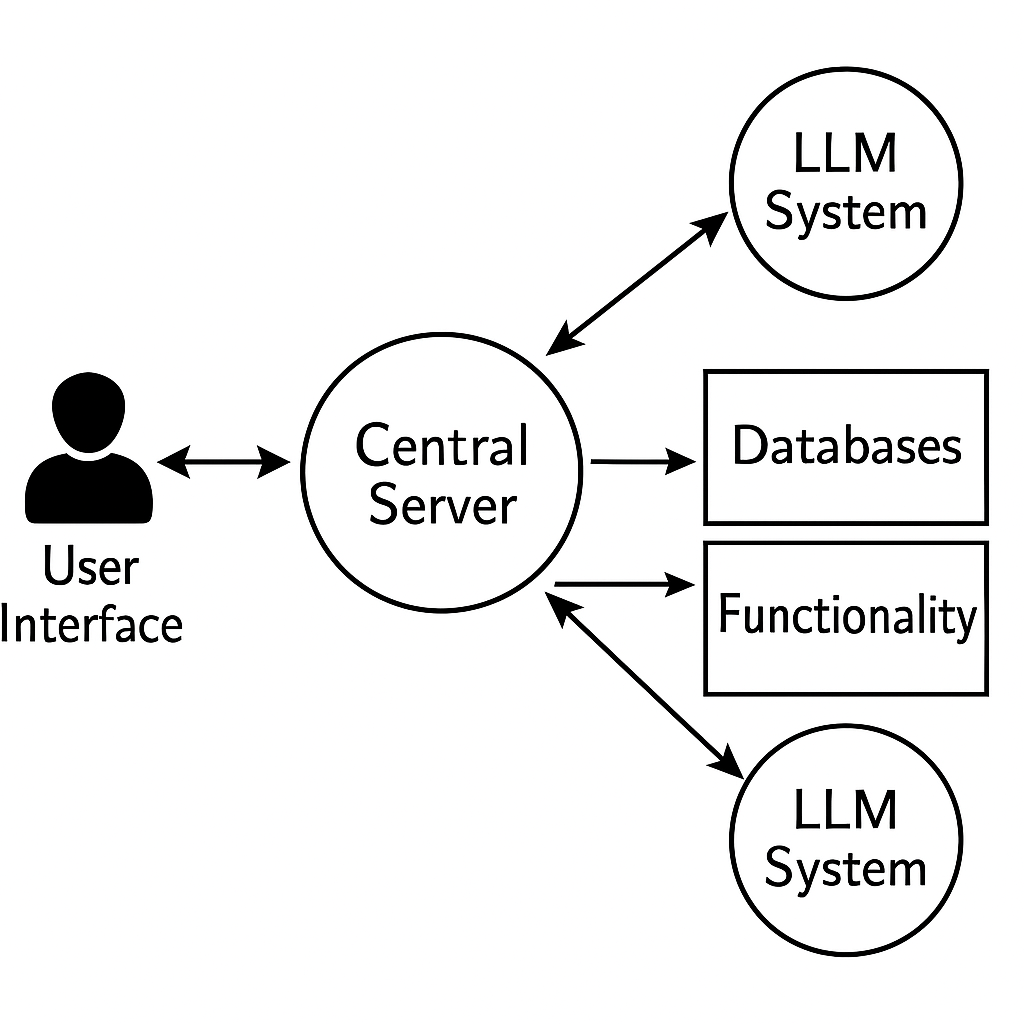
\includegraphics[width=0.5\textwidth]{images/user-server-database-llm.png}}
	\caption{How APIs are crucial for AI/ML applications involving large language models (LLM) with user services. The {\bf user interface} interacts with the {\bf central server} through an API. The server uses APIs to talk to the {\bf LLMs}. It uses APIs for {\bf database requests} (including the user and rights management, but also to pull observations, fields, analyses and much more. It also interacts with specific {\bf functionality} providing \textcolor{DWDblue}{\bf weather and climate services}, including sophisticated AI/ML applications, through further APIs.}
\end{figure}
\end{center}%

We have the full server code as demo application in the file \texttt{flask\_server\_request\_api.py}. Here, we explain its components: 

{\bf Server Setup.} We start by importing necessary modules and creating the Flask app instance.

\begin{codeonly}{Setup}
from flask import Flask, jsonify, request, abort, send_from_directory
from werkzeug.utils import secure_filename
import os

app = Flask(__name__)
\end{codeonly}

{\bf Upload Folder and Allowed Extensions.} Define the upload folder and allowed file types.

\begin{codeonly}{Upload Configuration}
UPLOAD_FOLDER = 'uploads'
ALLOWED_EXTENSIONS = {'txt', 'pdf', 'png', 'jpg', 'jpeg', 'gif'}

if not os.path.exists(UPLOAD_FOLDER):
    os.makedirs(UPLOAD_FOLDER)

def allowed_file(filename):
    return '.' in filename and \
           filename.rsplit('.', 1)[1].lower() in ALLOWED_EXTENSIONS
\end{codeonly}

{\bf In-Memory Item List.} A simple list of items simulates a database.

\begin{codeonly}{Initial Items}
items = [
    {"id": 1, "name": "Item 1"},
    {"id": 2, "name": "Item 2"},
]
\end{codeonly}

{\bf GET /items.} Return all items.

\begin{codeonly}{GET /items}
@app.route('/items', methods=['GET'])
def get_items():
    return jsonify(items)
\end{codeonly}

{\bf GET /items/<id>.} Return a single item by ID.

\begin{codeonly}{GET /items/<id>}
@app.route('/items/<int:item_id>', methods=['GET'])
def get_item(item_id):
    item = next((item for item in items if item['id'] == item_id), None)
    if item is None:
        abort(404)
    return jsonify(item)
\end{codeonly}

{\bf POST /items.} Add a new item.

\begin{codeonly}{POST /items}
@app.route('/items', methods=['POST'])
def create_item():
    if not request.json or 'name' not in request.json:
        abort(400)
    new_item = {
        "id": items[-1]["id"] + 1 if items else 1,
        "name": request.json['name']
    }
    items.append(new_item)
    return jsonify(new_item), 201
\end{codeonly}

{\bf PUT /items/<id>.} Update or create an item by ID.

\begin{codeonly}{PUT /items/<id>}
@app.route('/items/<int:item_id>', methods=['PUT'])
def update_or_create_item(item_id):
    if not request.json or 'name' not in request.json:
        abort(400)
    item = next((item for item in items if item['id'] == item_id), None)
    if item is None:
        new_item = {"id": item_id, "name": request.json['name']}
        items.append(new_item)
        return jsonify(new_item), 201
    else:
        item['name'] = request.json.get('name', item['name'])
        return jsonify(item)
\end{codeonly}

{\bf DELETE /items/<id>.} Delete an item.

\begin{codeonly}{DELETE /items/<id>}
@app.route('/items/<int:item_id>', methods=['DELETE'])
def delete_item(item_id):
    global items
    items = [item for item in items if item['id'] != item_id]
    return jsonify({'result': True})
\end{codeonly}

{\bf POST /items/<id>/upload.} Upload a file for a specific item.

\begin{codeonly}{POST /items/<id>/upload}
@app.route('/items/<int:item_id>/upload', methods=['POST'])
def upload_file(item_id):
    item = next((item for item in items if item['id'] == item_id), None)
    if item is None:
        abort(404)
    if 'file' not in request.files:
        abort(400, description="No file part in the request")
    file = request.files['file']
    if file.filename == '':
        abort(400, description="No selected file")
    if file and allowed_file(file.filename):
        filename = secure_filename(file.filename)
        saved_filename = f"{item_id}_{filename}"
        file_path = os.path.join(UPLOAD_FOLDER, saved_filename)
        file.save(file_path)
        item['file'] = file_path
        return jsonify({'result': 'File uploaded', 'file_path': file_path}), 201
    else:
        abort(400, description="File type not allowed")
\end{codeonly}

{\bf GET /items/<id>/download.} Download a file attached to an item.

\begin{codeonly}{GET /items/<id>/download}
@app.route('/items/<int:item_id>/download', methods=['GET'])
def download_file(item_id):
    item = next((item for item in items if item['id'] == item_id), None)
    if item is None or 'file' not in item:
        abort(404)
    file_path = item['file']
    directory, filename = os.path.split(file_path)
    return send_from_directory(directory, filename, as_attachment=True)
\end{codeonly}

{\bf Start the Server.} Run the application in debug mode.

\begin{codeonly}{Run Server}
if __name__ == '__main__':
    app.run(debug=True)
\end{codeonly}

This server code, which you can view in detail in \texttt{flask\_server\_request\_api.py}, serves as the API’s backend. The careful design ensures that the API is both stateless and uniform, allowing clients to interact predictably with the service.

\bigskip
\textbf{Interacting with the API Using \texttt{requests}:}\\
On the client side, \texttt{code012\_REST\_client.py} demonstrates how to use the \texttt{requests} library to make calls to our API. Let’s consider a few typical examples:

\begin{enumerate}
  \item \textbf{Retrieving All Items:}\\  
  A simple GET request is used to fetch the list of items. The client code sends:
  \begin{verbatim}
response = requests.get('http://127.0.0.1:5000/items')
print(response.json())
  \end{verbatim}
  This call returns a JSON array containing all items. By decoding the response, the client can easily process and display the data.

  \item \textbf{Retrieving a Specific Item:}\\  
  To fetch an individual item, the client sends a GET request with the item’s ID in the URL:
  \begin{verbatim}
response = requests.get('http://127.0.0.1:5000/items/1')
print(response.json())
  \end{verbatim}
  If the item exists, the server returns its details in JSON format; if not, an error (typically a 404 Not Found) is returned.

  \item \textbf{Adding a New Item:}\\  
  The POST request is used to create a new item. In our implementation, the client sends a JSON payload:
  \begin{verbatim}
new_item = {'name': 'New Item'}
response = requests.post('http://127.0.0.1:5000/items', json=new_item)
print(response.json())
  \end{verbatim}
  The server then generates a new item with a unique ID and returns it. Notice that the \texttt{json=} parameter in the request call makes it easy to send JSON data without manual serialization.

  \item \textbf{Updating and Deleting Items:}\\  
  Similarly, PUT requests are used to update an item and DELETE requests to remove it. The corresponding code in \texttt{code012\_REST\_client.py} handles these actions by specifying the correct URL endpoints and sending appropriate JSON data if necessary.
	
	\item \textbf{Upload Functionality:}\\  
In addition to updating and deleting items, the REST API example demonstrates file uploads. Clients can attach files to specific items by sending a POST request to an endpoint such as \texttt{/items/\textless id\textgreater/upload}. This endpoint accepts multipart form-data where the file is provided under a designated field (e.g., \texttt{'file'}). On the server side, Flask processes the incoming file, ensures its name is secured using \texttt{secure\_filename}, and then saves it into a dedicated uploads directory. The file path is subsequently stored in the item's record, associating the file with the item. This approach enables users to easily manage additional resources related to each item.

\item \textbf{Download Functionality:}\\  
Complementing the upload feature, the API also provides a download endpoint at \linebreak\texttt{/items/\textless id\textgreater/download}. When a client sends a GET request to this endpoint, the server locates the file associated with the item and transmits it back as an attachment using Flask's \texttt{send\_from\_directory} function. This not only ensures that the file is delivered with the correct MIME type but also prompts the client’s browser to download it rather than display it inline. On the client side, the downloaded file can be saved with its original name by removing any item-specific prefixes that were added during upload, thus preserving the original filename. This integrated upload and download mechanism enhances the functionality of the REST API by allowing it to handle both data and associated file resources seamlessly.

\end{enumerate}

\begin{codeonly}{}
import requests

# Base URL of the API
base_url = 'http://127.0.0.1:5000'

# GET all items
response = requests.get(f'{base_url}/items')
print("GET /items:", response.json())

# GET a specific item (e.g., id = 1)
response = requests.get(f'{base_url}/items/1')
print("GET /items/1:", response.json())

# POST a new item
new_item = {'name': 'New Item'}
response = requests.post(f'{base_url}/items', json=new_item)
print("POST /items:", response.json())

# PUT to update an item (e.g., id = 1)
updated_item = {'name': 'Updated Item 1'}
response = requests.put(f'{base_url}/items/1', json=updated_item)
print("PUT /items/1:", response.json())

# DELETE an item (e.g., id = 1)
response = requests.delete(f'{base_url}/items/1')
print("DELETE /items/1:", response.json())

# Check items after deletion
response = requests.get(f'{base_url}/items')
print("GET /items after deletion:", response.json())

# -------------------------
# UPLOAD a file for an item (e.g., for item with id = 2)
upload_url = f'{base_url}/items/2/upload'
# Ensure you have a file named 'example.txt' in your current directory
with open('example.txt', 'rb') as f:
    files = {'file': f}
    response = requests.post(upload_url, files=files)
    print("POST /items/2/upload:", response.json())

# -------------------------
# DOWNLOAD the file associated with an item (e.g., for item with id = 2)
download_url = f'{base_url}/items/2/download'
response = requests.get(download_url, stream=True)
if response.status_code == 200:
    # Save the downloaded file locally
    with open('downloaded_example.txt', 'wb') as f:
        for chunk in response.iter_content(chunk_size=8192):
            f.write(chunk)
    print("File downloaded successfully and saved as downloaded_example.txt")
else:
    print("Failed to download file, status code:", response.status_code)
\end{codeonly}


\textbf{Error Handling and Debugging:}\\
A crucial aspect of making API requests is managing errors gracefully. The client code checks the HTTP status code returned by the server and handles error responses appropriately. For instance, if a GET request for an item returns a 404 status code, the client can notify the user that the requested item does not exist. Similarly, for POST and PUT requests, verifying that the server returns the expected 201 or 200 status code helps ensure that operations have completed successfully.

\bigskip

\textbf{Benefits of This Approach:}\\
Using the \texttt{requests} library to interact with our REST API provides several benefits:
\begin{itemize}
  \item \textbf{Simplicity:} The \texttt{requests} library offers an intuitive API that abstracts the complexity of HTTP communication.
  \item \textbf{Flexibility:} Developers can easily extend the client to support additional endpoints or incorporate authentication mechanisms.
  \item \textbf{Maintainability:} By separating the server (\texttt{code011\_REST.py}) and client (\texttt{code012\_REST\_client.py}) code, our architecture is modular. This makes it easier to update one component without affecting the other.
  \item \textbf{Reusability:} The external code inclusion method using \texttt{\textbackslash includeexternalcode} promotes code reuse and ensures that our documentation is consistent with our source code.
\end{itemize}

It is now very easy to define simple functions such as \texttt{list()}, \texttt{up(<filename>,<id>)} or \texttt{down(<id>)} to list all uploaded items, to upload a particular file or to download a particular file. 

\bigskip
In summary, making API requests with Python’s \texttt{requests} library is both straightforward and powerful. Our implementation demonstrates a complete cycle: setting up a REST API server with Flask, handling standard HTTP methods, and interacting with the API via a client script. The combination of clear server endpoints, robust client-side error handling, and modular code inclusion makes this approach a solid foundation for building scalable and maintainable web services.

\bigskip

By following these practices, you can build reliable applications that communicate over HTTP in a standardized way, ultimately leading to more effective and efficient software systems.

\begin{recommendationbox}
An API-centric mindset greatly enhances fast development, modular design, and clean separation of responsibilities.
\end{recommendationbox}

%================================================================================
%
%================================================================================
\section{Fortran Integration using \texttt{ctypes} as API}

In this section, we illustrate an approach to integrating FORTRAN code with Python by using the \texttt{ctypes} module. The library \texttt{ctypes} provides explicit control over data types and memory management when interfacing with compiled shared libraries.

\begin{center}
\begin{figure}[ht]
   \centerline{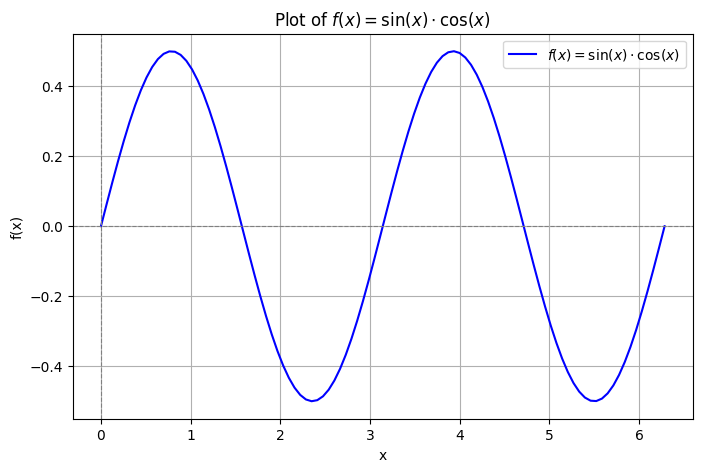
\includegraphics[width=0.6\textwidth]{images/sin_cos.png}}
	\caption{We use the Fortran \texttt{iso\_c\_binding module} to create a C-compatible API, allowing Fortran routines to be called from C or other languages such as Python via ctypes or f2py.}
\end{figure}
\end{center}%

The following example demonstrates how to load a Fortran shared library (compiled as \linebreak\texttt{fortran\_interface.so}), define the function prototype for the Fortran function \texttt{f\_sin\_cos}, and compute the function \( f(x) = \sin(x) \cdot \cos(x) \) for 100 values between 0 and \(2\pi\). The computed values are then plotted using Matplotlib. Additionally, the code checks for the existence of a Fortran debug log and prints its contents if available.

%\includeexternalcode{Fortran Module: code013\_fortran\_interface.f90}{code013_fortran_interface.f90}
\begin{codeonly}{FORTRAN code example}
%%writefile fortran_interface.f90
module fortran_module
    use iso_c_binding, only: c_double
    implicit none
contains
    function f_sin_cos(x) result(f) bind(C, name="f_sin_cos")
        implicit none
        real(c_double), intent(in) :: x
        real(c_double) :: f
        f = sin(x) * cos(x)
    end function f_sin_cos
end module fortran_module
\end{codeonly}

Compile this based on gfortran. 

\begin{codeonly}{Compilation}
gfortran -shared -fPIC fortran_interface.f90 -o fortran_interface.so
\end{codeonly}

Then, you might use the code, e.g.\ in a jupyter notebook or as basic python application. 

It can be extremely helpful to make your fortran modules and functions available for execution in your python framework. We will pursue this further in upcoming parts of this tutorial.

%================================================================================
%
%================================================================================


